\chapter{Σχετική Εργασία στην Αρχιτεκτονική} 
\label{chap:Literature}

\section{Σχετική Εργασία}

Τα τελευταία χρόνια γίνεται μια προσπάθεια να τυποποιηθούν τα 
peer-to-peer συστήματα σε μια ενιαία αρχιτεκτονική. Πιο γενικά σε ένα 
μοντέλο αναφοράς όπου περιγράφονται βασικές οντότητες και 
αλληλεπιδράσεις και βάσει αυτού μπορούν να κατασκευαστούν τέτοια 
συστήματα.

Στην δημοσίευση \citep{F.Dabek2003} έχουμε τον διαχωρισμό του συστήματος 
σε τρία επίπεδα. Το πρώτο επίπεδο αφορά την δρομολόγηση η οποία βασίζεται σε κλειδιά 
(key-based routing). Πάνω σε αυτό χτίζονται τα πρωτόκολλα του συστήματος 
\begin{wrapfigure}{l}{0.5\textwidth}
  \begin{center}
    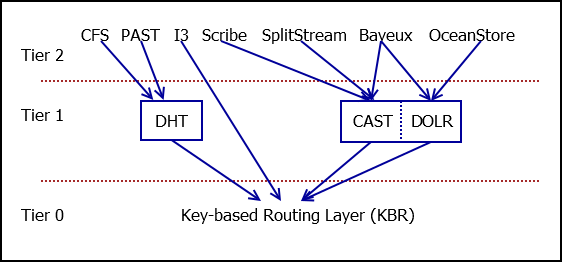
\includegraphics[width=0.48\textwidth]{Figures/Related_work/Towards_a_common_API_(tiers).png}
  \end{center}
  \caption{Towards a common API}
  \label{fig:Α_common_API}
\end{wrapfigure}
όπως κατανεμημένοι πίνακες κατακερματισμού (DHT), αποκεντρωμένη 
τοποθεσία αντικειμένου και δρομολόγησης (Decentralized Object Location 
and Routing) καθώς και anycast/multicast λειτουργικότητα. Οι εφαρμογές 
έχουν πρόσβαση που αποτελούν το ανώτερο αρχιτεκτονικό επίπεδο, έχουν 
πρόσβαση απευθείας στα δυο κατώτερα επίπεδα. Οι διεπαφές που 
προτείνονται όμως δεν μπορούν να καλύψουν όλες τις ανάγκες. Στο σχήμα  
\ref{fig:Α_common_API} φαίνονται τα επίπεδα της προτεινόμενης αρχιτεκτονικής.

Ο εμπνευστής του PGrid συστήματος με την ομάδα του εισάγει ένα 
μοντέλο αναφοράς \citep{Aberer05theessence} στο οποίο μπορούν να σχεδιαστούν 
διάφορα peer-to-peer συστήματα. Στο σχήμα \ref{fig:Essence} παρουσιάζονται τα 
αρχιτεκτονικά επίπεδα του μοντέλου. Στηρίζεται πάνω στο επίπεδο του 
δικτύου το οποίο συγκεντρώνει τα πρωτόκολλα   
\begin{wrapfigure}{l}{0.45\textwidth}
  \begin{center}
    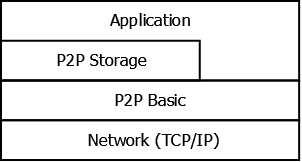
\includegraphics[width=0.43\textwidth]{Figures/Related_work/The_essence_of_p2p_(architecture).png}
  \end{center}
  \caption{Προτεινόμενη αρχιτεκτονική από Aberer et al.}
  \label{fig:Essence}
\end{wrapfigure}
TCP/IP. Αυτό παρέχει τις λειτουργίες του στο βασικό επίπεδο (P2P basic) το οποίο και υλοποιεί το 
peer-to-peer δίκτυο. Οι λειτουργίες που παρέχει είναι η σύνδεση (join) 
και η αποχώρηση (leave) στο δίκτυο, αναζήτησης (lookup) και δρομολόγησης 
(route). Στη συνέχεια έχουμε το επίπεδο αποθήκευσης (P2P storage) που 
παρέχει λειτουργίες εισαγωγής (insert), διαγραφής (delete), ανανέωσης 
(update) δεδομένων στο δίκτυο καθώς και τη διενέργεια ερωτήσεων πάνω σε 
αυτά (query). Για την ανάπτυξη μιας εφαρμογή, χρησιμοποιούνται οι 
διεπαφές που προσφέρονται από το βασικό επίπεδο και αυτό της 
αποθήκευσης. Στο σχήμα \ref{fig:Essence_UML} παρουσιάζεται το 
προτεινόμενο βασικό μοντέλο.

\begin{figure}[htbp]
  \begin{center}
    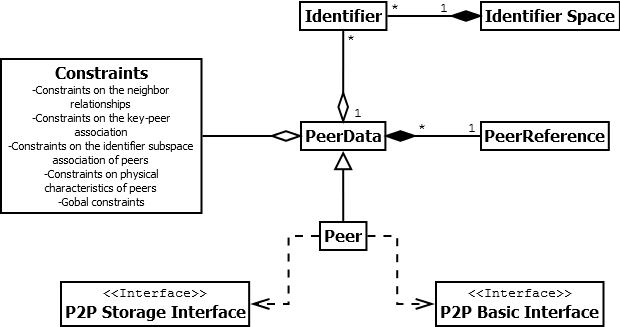
\includegraphics[scale=0.55]{Figures/Related_work/The_essence_of_p2p_(uml).png}
  \end{center}
  \caption{Προτεινόμενο μοντέλο αναφοράς από Aberer et al.}
  \label{fig:Essence_UML}
\end{figure}

Σε αυτό φαίνονται τα απαραίτητα συστατικά που προκύπτουν από την 
ανάλυση, οι διάφοροι περιορισμοί που τίθενται και οι διεπαφές που πρέπει 
να υποστηρίζει κάθε peer-to-peer σύστημα. Στην υλοποίηση του PGrid από 
τον Schmidt \citep{Schmidt2007}, ακολουθήθηκε το παραπάνω 
μοντέλο. Η όλη λογική είναι ένα peer-to-peer σύστημα να είναι χαλαρά 
συνδεδεμένο με τις υπηρεσίες που προσφέρουν το βασικό επίπεδο και αυτό 
της αποθήκευσης. Στόχος είναι η ευκολία αλλαγής συμπεριφοράς του ίδιου 
συστήματος εναλλάσσοντας τις διάφορες υλοποιήσεις. Παρόλα αυτά όπως 
προκύπτει από την εξέταση της υλοποίησης, είναι δύσκολο να επεκταθεί μια 
υπάρχουσα υλοποίηση με άλλα πρωτόκολλα πιο πολύπλοκα.

\begin{wrapfigure}{L}{0.5\textwidth}
  \begin{center}
    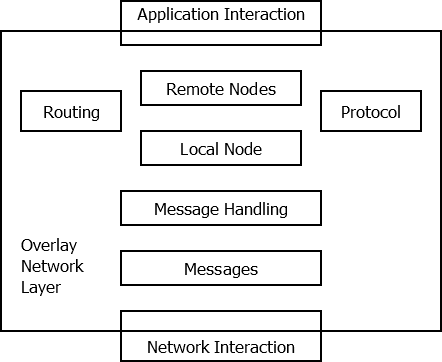
\includegraphics[width=0.48\textwidth]{Figures/Related_work/A_pattern_language.png}
  \end{center}
  \caption{A Pattern Language}
  \label{fig:Patterns}
\end{wrapfigure}

Για την εσωτερική δομή επιπέδων όπως αυτό του βασικού της παραπάνω 
αρχιτεκτονικής , έχουμε μια προσπάθεια να δημιουργηθούν σχεδιαστικά 
πρότυπα. Στις δημοσιεύσεις \citep{Grolimund2005, Grolimund2006} αναλύονται 
ένα σύνολο peer-to-peer συστημάτων και ενδιάμεσου λογισμικού. Από αυτό 
προκύπτουν σχεδιαστικά πρότυπα που έχουν να κάνουν με ένα βασικό στοιχείο 
αυτών των συστημάτων που είναι η δρομολόγηση των μηνυμάτων μέσα στο δίκτυο. 
Στο σχήμα \ref{fig:Patterns} φαίνεται η αρχιτεκτονική δομή του συγκεκριμένου επιπέδου. 
Κάθε στοιχείο του επιπέδου περιλαμβάνει μια σειρά σχεδιαστικών προτύπων. 

Στη δημοσίευση \citep{Amoretti2005} εισάγεται η έννοια 
του Peer ως σχεδιαστικό πρότυπο. Το πρόβλημα που προσπαθεί να επιλυθεί 
είναι η αποτελεσματική κατανομή του φόρτου εργασίας και η υψηλή 
διαθεσιμότητα των πόρων. Η λογική είναι παρόμοια μόνο που πλέον οι πόροι 
και οι λειτουργίες που προσφέρει ένας peer παρουσιάζονται ως υπηρεσίες. 
Ενδιαφέρει ο τρόπος με τον οποίο περιγράφονται οι υπηρεσίες και 
προτείνεται η ύπαρξη είτε μιας WSDL διεπαφής όπου μπορεί να ανακτηθεί 
πλήρως η λειτουργικότητα της είτε OWL-S περιγραφών σε περίπτωση που 
είναι αναγκαία η σημασιολογική περιγραφή (semantic) της πληροφορίας. 
Προτείνεται, μάλιστα, η χρήση Web Service αρχιτεκτονικής δεδομένου των 
πλεονεκτημάτων που μπορεί να φέρει μια τέτοια υπηρεσία. 

Από την πρακτική εφαρμογή του προτύπου \citep{Amoretti2005SP2A}. 
Χρησιμοποιήθηκαν τεχνολογίες όπως η JXTA και Web Services. Για την ανάπτυξη 
των τελευταίων χρησιμοποιήθηκαν τα JXTA-SOAP και OWL-S. Η περιγραφή των web 
service μέσω OWL-S κάνει εύκολη την ανακάλυψη, την εκτέλεση, την σύνθεση 
αυτών και την παρακολούθηση τους (monitoring). Παρόλα αυτά, το συγκεκριμένο 
framework υποστηρίζει υβριδικά και καθαρά peer-to-peer δίκτυα χωρίς όμως να 
υπάρχει συγκεκριμένη τοπολογία. Επίσης, δεν υπάρχει η έννοια της 
σύνθεσης των υπηρεσιών στο ίδιο το λογισμικό του peer σε πιο πολύπλοκες 
διαδικασίες/πρωτόκολλα.

Σημαντική δουλειά είναι τα JXTA πρωτόκολλα \citep{JXTA2007}. Αυτά 
αποτελούν μια ανοιχτή διαδικτυακή πλατφόρμα για peer-to-peer συστήματα. 
Τυποποιείται ο τρόπος με τον οποίο ένας peer ανακαλύπτει άλλους, πώς 
οργανώνεται σε ομάδες peer και πως επικοινωνεί. Επίσης, ορίζονται 
πρωτόκολλα για την διαφήμιση και ανακάλυψη διαδικτυακών πόρων. Υπάρχουν 
τρία αρχιτεκτονικά επίπεδα με πρώτο το επίπεδο της πλατφόρμας όπου 
ορίζονται κλασικοί τύποι για ένα peer-to-peer δίκτυο. Στη συνέχεια 
έχουμε το επίπεδο των υπηρεσιών το οποίο περιλαμβάνει διαδικτυακές 
υπηρεσίες όπως αναζήτησης και ευρετηριοποίησης, αποθηκευτικού χώρου, 
διαμοιρασμού αρχείων, κατανεμημένα συστήματα αρχείων και άλλα. Το τελικό 
επίπεδο είναι αυτό της εφαρμογής που εκμεταλλεύεται τις προσφερόμενες 
υπηρεσίες. Δεν υπάρχει όμως καθορισμός της τοπολογίας των peer-to-peer 
δικτύων που προκύπτουν και τα πρωτόκολλα είναι ορισμένα ως ένα σύνολο 
από XML μηνύματα προκειμένου την ανεξαρτητοποίηση από λειτουργικά 
συστήματα και γλώσσες προγραμματισμού.
